%143


\section{プログラミングの\ruby{復習}{ふく|しゅう}をしよう}

\subsection{\ruby{作業}{さ|ぎょう}フォルダの\ruby{準備}{じゅん|び}}
\bigskip
\bigskip

上にあるバーのアイコンからファイルマネージャーを開いてみましょう。


\begin{figure}[H]
  \begin{center}
    
\includegraphics[keepaspectratio,width=5.898cm,height=1.242cm]{text04-img/text02-img001.png}
    \caption{ファイルマネージャーを開くアイコン}
  \end{center}
  \label{fig:prog_menu}
\end{figure}

これから作業で使うファイルをコピーしてもらいます。「/home/ユーザー名」のフォルダに、第4回で使うフォルダ「04」をコピーすることから始めます。

まず、「/usr/local/share/ome」という場所を開いてみましょう。

どこにあるか探すことができますか?

わからない時は、TAや先生に聞いてみましょう。


\begin{figure}[H]
  \begin{center}
    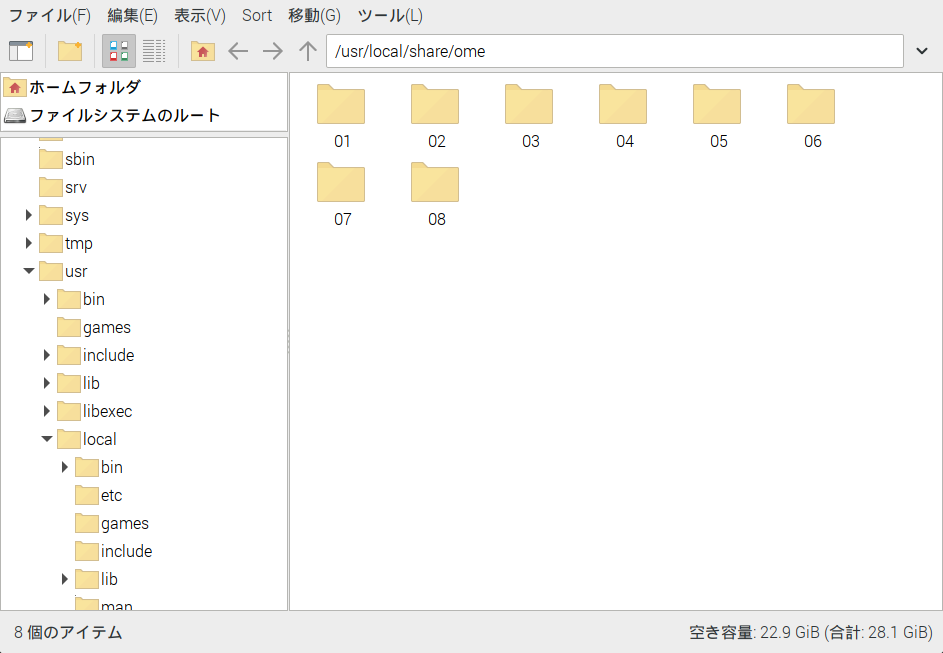
\includegraphics[keepaspectratio,width=11.232cm,height=8.424cm]{text04-img/s_ome04a.png}
    \caption{/usr/local/share/ome フォルダ}
  \end{center}
  \label{fig:prog_menu}
\end{figure}

この中に、「04」という名前のフォルダがあります。これから、この「04」というフォルダを自分の作業フォルダにコピーします。

「04」という名前のフォルダ上でマウスの右クリックを押して「コピー」を選んでください。

%195

\begin{figure}[H]
  \begin{center}
    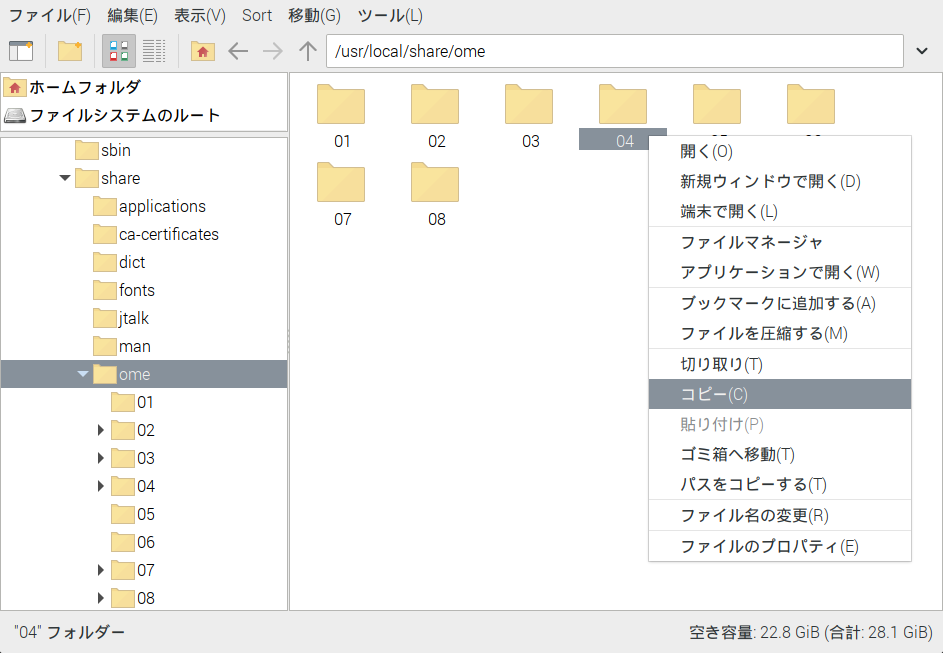
\includegraphics[keepaspectratio,width=11.232cm,height=8.424cm]{text04-img/s_ome04b.png}
    \caption{04フォルダでコピーを選ぶところ}
  \end{center}
  \label{fig:prog_menu}
\end{figure}



コピーを選ぶだけでは何も起こりません。この後、コピーしたい場所を選びます。

コピー先の場所は、「/home/ユーザー名」のフォルダになります。

たとえば、ユーザー名が「ome」だった場合は、「/home/ome」という場所にコピーします。

コピー先の場所を開いたら、何もない場所でマウスの右クリックを押して「貼り付け」を選んでください。



\begin{figure}[H]
  \begin{center}
    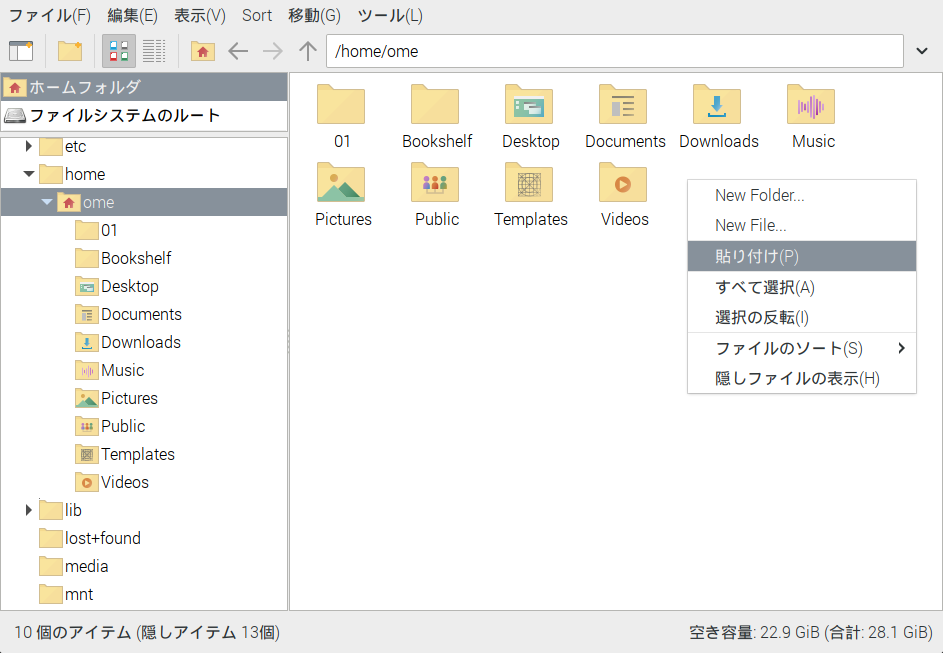
\includegraphics[keepaspectratio,width=11.232cm,height=8.424cm]{text04-img/s_ome04c.png}
    \caption{04フォルダでコピーを選ぶところ}
  \end{center}
  \label{fig:prog_menu}
\end{figure}


これで先ほどの「/usr/local/share/ome/04」フォルダが、「/home/ユーザー名/04」にコピーされます。

ファイルには、画像や文章、音声や動画など、さまざまなデータが入っています。

これから皆さんが作業で使うファイルは、「/home/ユーザー名/04」という場所に置かれています。

ファイルの中身が何なのか、自分が作ったファイルかどうかを知っておいてください。



\begin{figure}[H]
  \begin{center}
    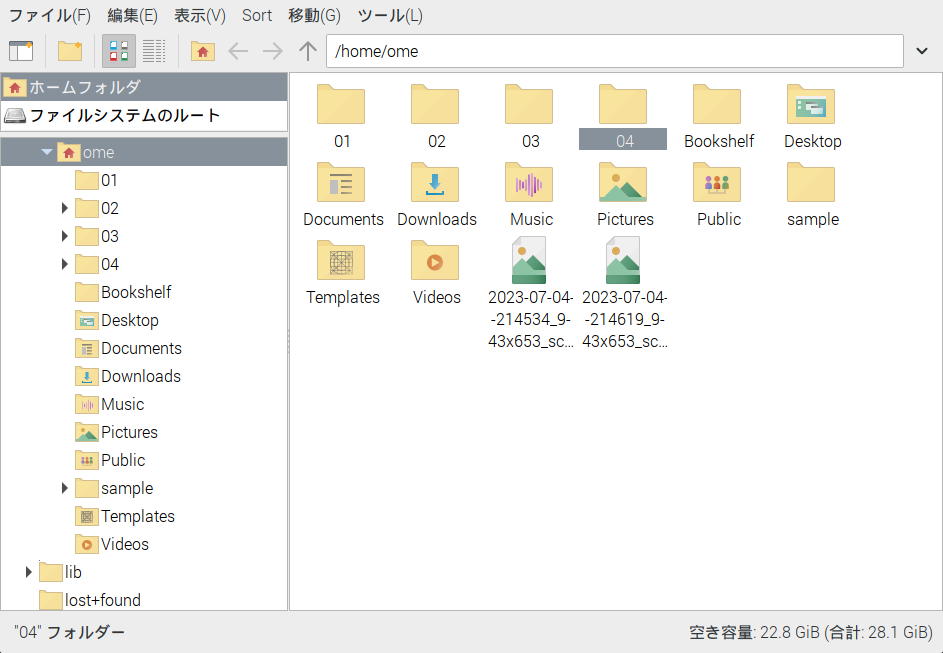
\includegraphics[keepaspectratio,width=11.232cm,height=8.424cm]{text04-img/s_ome04d.png}
    \caption{04フォルダがコピーされた画面}
  \end{center}
  \label{fig:prog_menu}
\end{figure}





